\documentclass[12pt]{article}
\usepackage{graphicx}
\usepackage{xcolor}
\usepackage{hyperref}
\usepackage{wasysym}
\usepackage{mathrsfs}
\usepackage[calc]{datetime2}
\usepackage{boondox-cal}
\usepackage{bm} % For bold math symbols
\usepackage{amsmath,amsthm,amssymb,amsbsy}
\usepackage{gensymb}
\usepackage{cancel}
\usepackage{tikz}
\usetikzlibrary{3d,calc}
\usetikzlibrary{arrows}

\DTMsavenow{now}
\DTMsavedate{DueDate}{2024-03-12}

\newcount\daystilldue
\newcount\hourstilldue
\newcount\minutestilldue

% Calculate the difference in days
\DTMsaveddatediff{DueDate}{now}{\daystilldue}

% Calculate the difference in hours and minutes
\hourstilldue=\DTMfetchhour{DueDate}
\advance\hourstilldue by -\DTMfetchhour{now}
\minutestilldue=\DTMfetchminute{DueDate}
\advance\minutestilldue by -\DTMfetchminute{now}

% Adjust for negative values
\ifnum\hourstilldue<0
  \advance\hourstilldue by 24
  \advance\daystilldue by -1
\fi
\ifnum\minutestilldue<0
  \advance\minutestilldue by 60
  \advance\hourstilldue by -1
\fi

\newcommand{\TimeUntilDue}{
  \ifnum\daystilldue<4
    \textcolor{red}{
    \number\daystilldue\ days - 
    \number\hourstilldue\ hours - 
    \number\minutestilldue\ min until deadline!!
  }
\else
    \number\daystilldue\ days - 
    \number\hourstilldue\ hours - 
    \number\minutestilldue\ min until deadline
  \fi
}



% Save the original \BibTeX command in case you need it later
\let\originalBibTeX\BibTeX

% Redefine the \BibTeX command to display the LaTeX logo
\renewcommand{\BibTeX}{{\rmfamily B\kern-.03em{\sffamily ib}\kern-.15em\TeX}}


\newcommand{\delCross}[1]{
  \left[\hat a_x\left(\frac{\partial\bm{#1}_z}{\partial y} - \frac{\partial\bm{#1}_y}{\partial z}\right) - \hat a_y\left( \frac{\partial\bm{#1}_z}{\partial x} - \frac{\partial\bm{#1}_x}{\partial z}  \right) + \hat a_z\left( \frac{\partial\bm{#1}_y}{\partial x} -  \frac{\partial\bm{#1}_x}{\partial y}\right)\right]
}
\begin{document}

\newcommand{\Cross}[2]{
\hat a_x(#1_2#2_3 -#1_3#2_2) -\hat a_y(#1_1#2_3-#1_3#2_1) + \hat a_z(#1_1#2_2-#1_2#2_1) 
}
\title{ECE 6310 - Advanced Electromagnetic Fields: Homework Set \#4}
\author{Miguel Gomez}
\date{\TimeUntilDue}
\maketitle

%\begin{center}
%  $\mathcal{ABCDEFGHIJKLMNOPQRSTUVWXYZ}$\\
%$\mathscr{ABCDEFGHIJKLMNOPQRSTUVWXYZ}$
%\end{center}
\section*{Preliminaries}
In this document, we use standard notation for electromagnetic theory. Key equations and concepts are summarized below:

\subsection*{Vector Notation}
\begin{itemize}
  \item $\bm{\mathcal{E}}$: Electric field intensity
  \item $\bm{\mathcal{H}}$: Magnetic field intensity
  \item $\bm{\mathcal{D}}$: Electric flux density
  \item $\bm{\mathcal{B}}$: Magnetic flux density
  \item $\bm{\mathcal{J}}$: Current density
  \item $\rho_v$: Volume charge density
\end{itemize}

\subsection*{Differential Operators}
\begin{itemize}
  \item $\nabla \cdot\ \ $: Divergence of a vector field
  \item $\nabla \times\ \ $: Curl of a vector field
  \item $\nabla\ \ $: Gradient of a scalar field
  \item $\partial_i\ \ $: Partial derivative with respect to the independent basis element $i$
\end{itemize}

\subsection*{Maxwell's Equations}
In integral form, Maxwell's equations are given by:
\begin{align}
  \oint_{\partial V} \bm{\mathcal{E}} \cdot d\bm{\mathcal{l}} &= - \frac{d}{dt} \int_{V} \bm{\mathcal{B}} \cdot d\bm{\mathcal{S}} & \text{(Faraday's Law of Induction)} \\
  \oint_{\partial V} \bm{\mathcal{H}} \cdot d\bm{\mathcal{l}} &= \int_{V} \bm{\mathcal{J}} \cdot d\bm{\mathcal{S}} + \frac{d}{dt} \int_{V} \bm{\mathcal{D}} \cdot d\bm{\mathcal{S}} & \text{(Ampère's Circuital Law)} \\
  \oiint_{\partial V} \bm{\mathcal{D}} \cdot d\bm{\mathcal{S}} &= \int_{V} \rho_v dV & \text{(Gauss's Law for Electricity)} \\
  \oiint_{\partial V} \bm{\mathcal{B}} \cdot d\bm{\mathcal{S}} &= 0 & \text{(Gauss's Law for Magnetism)}
\end{align}

\subsection*{Other Relevant Equations}
\begin{itemize}
  \item Continuity Equation: $\nabla \cdot \bm{\mathcal{J}} + \partial_t \rho_v = 0$
  \item Relationship between $\bm{\mathcal{E}}$, $\bm{\mathcal{D}}$: $\bm{\mathcal{D}} = \epsilon \bm{\mathcal{E}}$
  \item Relationship between $\bm{\mathcal{H}}$, $\bm{\mathcal{B}}$: $\bm{\mathcal{B}} = \mu \bm{\mathcal{H}}$
\end{itemize}

\subsection*{Boundary Conditions}
Discuss the boundary conditions for $\bm{\mathcal{E}}$, $\bm{\mathcal{H}}$, $\bm{\mathcal{D}}$, and $\bm{\mathcal{B}}$ at interfaces between different media.
\newpage
\section{- 8.2}
A standard X-band ($8.2–12.4 GHz$) rectangular waveguide with inner dimensions of 0.9 in. ($2.286\ cm$) by 0.4 in. ($1.016\ cm$) is filled with lossless polystyrene ($\epsilon_r = 2.56$). For the lowest-order mode of the waveguide, determine at $10 GHz$ the following values.
\begin{itemize}
\item[(a)] Cutoff Freq ($f_c$) in $GHz$\\
  We can find this with expression (8-16) from \cite{balanis_2012} with $a = 2.286\ cm$.
  \begin{align*}
    (f_{c})_{mn} &= \frac{1}{2\pi\sqrt{\mu\epsilon}}\sqrt{\left(\frac{m\pi}{a}\right)^2 + \left(\frac{n\pi}{b}\right)^2}\\
    (f_{c})_{10}  &= \frac{1}{2\pi\sqrt{\mu\epsilon}}\sqrt{\left(\frac{1\pi}{a}\right)^2 + \left(\frac{0\pi}{b}\right)^2}\\
                 &= \frac{1}{2\pi\sqrt{\mu\epsilon}}\sqrt{\left(\frac{\pi}{a}\right)^2}\\
    &= \frac{1}{2\pi\sqrt{\mu\epsilon}}\sqrt{\left(\frac{\pi}{2.86*10^{-2}}\right)^2} = 4.09832 GHz
  \end{align*}
\item[(b)] Guide wavelength ($\lambda_g$) in $cm$\\
  This one can be done with a combination of expressions from chapter 8 in \cite{balanis_2012}, (8-21a,b,c). we can do this with $a$ because the frequency in question is $10GHz$ which us above the cutoff found in part $a$.
  \begin{align*}
    (\lambda_g)_{mn} &= \frac{\lambda}{\sqrt{1-\left(\frac{f_c}{f}\right)^2}}\\
                     &= \frac{\lambda}{\sqrt{1-\left(\frac{4.09832e^{9}}{1e^{10}}\right)^2}}\\
                     &= \frac{0.0187375}{\sqrt{1-\left(.409832\right)^2}}\\
                     &= 0.0205419\ [m] = 2.05419\ [cm]
  \end{align*}
\item[(c)] Wave impedance ($\eta$)\\
  This can be found with (8-20a) in \cite{balanis_2012}.
  \begin{align*}
    Z_w^+ &= \frac{\sqrt{\frac{\mu}{\epsilon}}}{\sqrt{1-\left(\frac{f_c}{f}\right)^2}} = \frac{\eta}{\sqrt{1-\left(\frac{f_c}{f}\right)^2}}\\
    Z_w^+ &= \frac{\sqrt{\frac{\mu_0}{\epsilon_0\epsilon_r}}}{\sqrt{1-\left(.409832\right)^2}} \\
    \eta_0 &= 120\pi\\
          &= \frac{\frac{\eta_0}{\sqrt{\epsilon_r}}}{\sqrt{1-\left(.409832\right)^2}} = \frac{120\pi}{\sqrt{2.56}\cdot 0.912161}\\
    &= 258.309\ \Omega
  \end{align*}
\item[(d)] Phase velocity ($v_p$) in $\frac{m}{s}$
\item[(e)] Group velocity in $\frac{m}{s}$ \\
  This velocity, as well as the group velocity, can be found using expression (8.49a-c) from \cite{balanis_2012}. These reduce to a simple expression in (8-52) 
  \begin{align*}
    v_p &= \frac{v}{\cos{(\Psi)}}\\
    v_g &= v\cos{(\Psi)}\\
    \Psi &= \cos{^{-1}\left(\sqrt{1-\left(\frac{f_c}{f}\right)^2}\right)}
  \end{align*}
  Since inverse $\cos$ returns an angle, taking the $\cos$ of the inverse is the argument to the inverse itself.
  \begin{align*}
    v_p &= \frac{v}{\sqrt{1-\left(\frac{f_c}{f}\right)^2}}\\
    v_g &= v\sqrt{1-\left(\frac{f_c}{f}\right)^2}
  \end{align*}
\end{itemize}
\newpage
\noindent
Since $v$ is the expression $\frac{c}{\sqrt{\epsilon_r}}$, we can input those into the expression and solve for the speeds.
  \begin{align*}
    v_p &= \frac{c}{\sqrt{\epsilon_r}\sqrt{1-\left(\frac{f_c}{f}\right)^2}} = 2.05419*10^8 \left[\frac{m}{s}\right] \\
    v_g &= \frac{c}{\sqrt{\epsilon_r}}\sqrt{1-\left(\frac{f_c}{f}\right)^2} = 1.70916*10^8 \left[\frac{m}{s}\right]
  \end{align*}

\section{- 9.14}
A circular waveguide with radius of $3 cm$ is made of copper ($\sigma = 5.76 × 107 \frac{S}{m}$). For the dominant $TE_{11}$ and low-loss $TE_{01}$ modes, determine their corresponding cut-off frequencies and attenuation constants (in $\frac{Np}{m}$ and $\frac{dB}{m}$ at a frequency of $7 GHz$. Assume that the waveguide is filled with air.

This problem can be modeled using CST, or Ansys, and we can also solve for the values directly. Using the expression for the cutoff frequency seen in 9-12a of \cite{balanis_2012}, we can solve for $f_c$, and using expression 9-34a in  \cite{balanis_2012}, we can solve for the attenuation constant for our modes. $\chi_{mn}'$ depends on the mode and can be found with table 9-1 of \cite{balanis_2012}.

\begin{align*}
  f_c &= \frac{\chi_{mn}'}{2\pi a \sqrt{\mu\epsilon}}\\
  \alpha_{mn} &= \frac{R_s}{a\eta\sqrt{1-\left(\frac{f_c}{f}\right)^2}}\left[ \left(\frac{f_c}{f}\right)^2 + \frac{m^2}{\chi_{mn}'^2- m^2}  \right]
\end{align*}
\begin{itemize}
\item[$TE_{11}$] : $\chi_{11}' = 1.8412$
  \begin{itemize}
    \item [a)] $f_c$
    \item [b)] $\alpha_c$\\
  \end{itemize}
  \item[$TE_{01}$] : $\chi_{01}' = 3.8318$
  \begin{itemize}
    \item [a)] $f_c$
    \item [b)] $\alpha_c$
  \end{itemize}
\end{itemize}
\newpage
\section{- 11.2}
A magnetic line source of infinite length and constant magnetic current Im is placed parallel to the z axis at a height h above a PEC ground plane of infinite extent, as shown in Figure 11-2 except that we now have a magnetic line source.
\begin{itemize}
\item[(a)] Determine the total magnetic field at $\rho$, $\phi$ for $0\le \phi \le 180\degree$.
\item[(b)] Simplify the expressions when the observations are made at very large distances (far field).
\item[(c)] Determine the smallest height $h$ (in $\lambda$) that will introduce a null in the far field amplitude pattern at:
  \begin{itemize}
  \item[\cdot] $\phi = 30\degree$
  \item[\cdot] $\phi = 90\degree$
  \end{itemize}
\end{itemize}
\begin{center}
\begin{figure}[h]
    \centering
    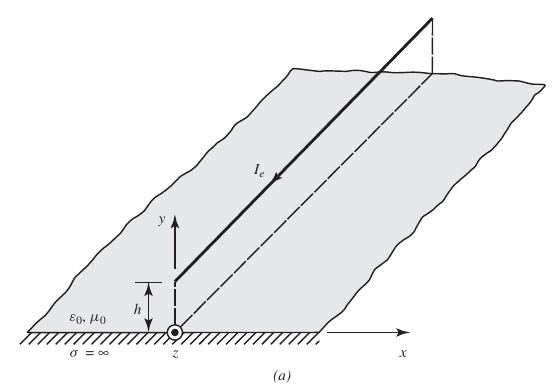
\includegraphics[width=10cm]{./images/fig11-2.png}
    \caption{fig. 11-2}
    \label{fig:11-2}
  \end{figure}
\end{center}

\newpage
\section{- 11.20}
For a strip of width $w = 2\lambda$, plot the $\frac{RCS}{\lambda_o^2}$ (in dB) when the length of the strip is $l = 5\lambda$, $10\lambda$ and $20\lambda$ (plot all three graphs on the same figure). Use the approximate relation between the 2D SW and the 3D RCS. Assume normal incidence.

\newpage

\bibliographystyle{plain}
\bibliography{references/references}

\end{document}

%%% Local Variables:
%%% mode: LaTeX
%%% TeX-master: t
%%% End:
